\documentclass[a4paper]{article}

\usepackage{indentfirst}
\usepackage{geometry}
\usepackage{graphicx}
\usepackage{makecell}
\usepackage[utf8]{inputenc}
\usepackage[russian]{babel} 

\geometry{left=0.8cm,right=0.8cm,top=3cm,bottom=3cm}

\begin{document}

\setlength{\parskip}{1em}

\begin{tabular}{|p{86mm}|p{86mm}|}

    \newcommand{\innertable}{
        \begin{tabular}{c|c|c|c|c|c}
            \hline
            $q$ & \makecell[c]{\rotatebox{90}{Приближенное} \rotatebox{90}{значение л}} & \makecell[c]{Верхним\\ граница\\абсолютной\\ погрешности} & $\Delta$ & $h$ & $\lambda$  \\
            \hline
            $1$ & $\frac{3}{1}$ & $\frac{1}{2}=0.5000$ & $0,1416$ & $0,1416$ & $3,5$\\
            $2$ & $\frac{6}{2}$ & $\frac{1}{4}=0,2500$ & $0,1416$ & $0,2832$ & $1,8$\\
            $3$ & $\frac{9}{3}$ & $\frac{1}{6}=0,1667$ & $0,1416$ & $0,4248$ & $1,2$\\
            $4$ & $\frac{13}{4}$ & $\frac{1}{8}=0,1250$ & $0,1084$ & $0,4336$ & $1.2$\\
            $5$ & $\frac{16}{5}$ & $\frac{1}{10}=0,1000$ & $0,1416$ & $0,2832$ & $1,7$\\
            $6$ & $\frac{19}{6}$ & $\frac{1}{12}=0,0833$ & $0,0251$ & $0,1504$ & $3,3$\\
            $7$ & $\frac{22}{7}$ & $\frac{1}{14}=0,0714$ & $0,0013$ & $0,0089$ & $56,5(!)$\\
            $8$ & $\frac{25}{8}$ & $\frac{1}{15}=0,0625$ & $0,0166$ & $0,1327$ & $3,8$\\
            $9$ & $\frac{28}{9}$ & $\frac{1}{18}=0,0556$ & $0,0305$ & $0,2743$ & $1,8$\\
            $10$ & $\frac{31}{10}$ & $\frac{1}{20}=0,0500$ & $0,0416$ & $0,4159$ & $1,2$\\
            \hline
        \end{tabular}
    }

    \ \ Величину\par $$\lambda=\frac{1}{2h}=\frac{1}{2|q\alpha-p|}$$\par назовем коэффициентом выгодности. Его смысл очень прост: коэффициент выгодности показывает, во сколько раз фактическая абсолютная погрешность меньше максимально возможной. Чем больше $\lambda$, тем выгоднее приближение.\par Очевидно,\par $$1\le\lambda<\infty,$$\par $$\lambda  h=\frac{1}{2}$$\par \ \ Не следует думать, что более мелкие доли всегда дают более точное приближение! Может случиться, что при нанесении на числовую ось восьмых долей число а занимает менее выгодное положение, чем при нанесении седьмых. Сделаем опыт с числом л, аппроксимируя его разными долями — от первых до десятых. Вычисления опущены, читатель может воспроизвести их сам.\par\ \par \innertable & \ \ Эта таблица показывает, что для аппроксимации л седьмые доли резко выгоднее ближайших соседних долей. Фактическая погрешность в 56 раз меньше, чем можно думать, судя по размеру долей *).\par \ \ На рисунке 2 показано расположение числа л на числовой оси. Случайно (а впрочем, случайно ли?) л оказывается очень близко к 3-~. Если бы нам заранее предписали аппроксимировать так, чтобы абсолютная\par 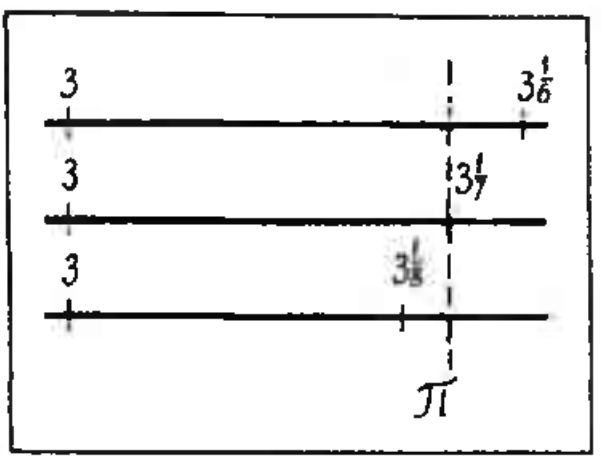
\includegraphics[scale=0.65]{pic 1}\par погрешность не превысила 0,0013, какие доли выбрали бы? Мы записали бы условие $\frac{1}{2q}\le 0,0013$ откуда $q\ge 385$, а Архимед достиг той же точности, взяв гораздо меньший знаменатель.\par \ \ Теперь вы убедились, читатель, что Архимед выбрал седьмые доли не случайно?\par \ \ Через много веков голландский математик Адриан Меций дал приближенное значение\par $$\pi=\frac{355}{113}$$\par Число Меция обладает теми же удивительными свойствами, что и числе Архимеда: знаменатель 113 гораздо\par ---------------\par *) Вычисление дает $\lambda=\frac{1}{2\cdot0,0089}=56,2.$\par Чтобы правильно получить цифры десятых, надо взять $h$ с пятью цифрами после запятой
  
\end{tabular}

\end{document}


